% !TeX program = pdflatex
\documentclass[border=6pt]{standalone}
\usepackage{amssymb}
\usepackage{tikz}
\usetikzlibrary{arrows.meta, positioning, calc, fit, backgrounds}

\definecolor{MediumRed}{rgb}{0.925, 0.345, 0.345}
\definecolor{MediumGreen}{rgb}{0.37, 0.7, 0.66}
\definecolor{MediumBlue}{rgb}{0.015, 0.315, 0.45}
\definecolor{DarkBlue}{rgb}{0.05, 0.15, 0.35}

\begin{document}
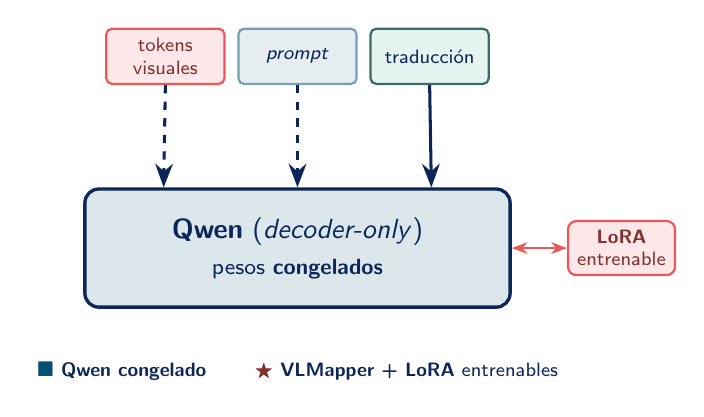
\begin{tikzpicture}[
    font=\sffamily,
    flow/.style={-{Stealth[length=3mm]}, line width=1.1pt, DarkBlue},
    tok/.style={draw, thick, rounded corners=2pt, minimum width=1.5cm, minimum height=0.7cm,
        font=\sffamily\scriptsize, align=center},
]

% ---- secuencia de entrada con mascara de perdida ----
\node[tok, draw=MediumRed, fill=MediumRed!14, text=MediumRed!55!black] (tv) at (0,0)
    {tokens\\visuales};
\node[tok, draw=MediumBlue!55, fill=MediumBlue!10, text=DarkBlue, right=0.15cm of tv] (tp) {\textit{prompt}};
\node[tok, draw=MediumGreen!60!black, fill=MediumGreen!16, text=DarkBlue, right=0.15cm of tp] (tt)
    {traducción};

% mascara
% \node[font=\sffamily\scriptsize, text=DarkBlue!55, below left= 0.05cm of tv] {$-100$ (ignorado)};
% \node[font=\sffamily\scriptsize, text=DarkBlue!55, below=0.1cm of tp] {$-100$ (ignorado)};
% \node[font=\sffamily\scriptsize\bfseries, text=MediumGreen!35!black, below=0.1cm of tt] {pérdida aquí};

% ---- Qwen ----
\node[draw=DarkBlue, very thick, rounded corners=5pt, fill=MediumBlue!14, text=DarkBlue,
      align=center, minimum width=5.4cm, minimum height=1.5cm, below=1.3cm of tp] (qwen)
    {\textbf{Qwen} (\textit{decoder-only})\\[1pt]\footnotesize pesos \textbf{congelados}};
\draw[flow, dashed] (tv.south) -- ($(qwen.north)+(-1.7,0)$);%++(0,-0.5) -| ($(qwen.north)+(-1.8,0)$);
\draw[flow, dashed] (tp.south) -- (qwen.north);
\draw[flow] (tt.south) -- ($(qwen.north)+(1.7,0)$);%++(0,-0.5) -| ($(qwen.north)+(1.8,0)$);

% ---- adaptadores LoRA ----
\node[draw=MediumRed, thick, rounded corners=3pt, fill=MediumRed!14, text=MediumRed!55!black,
      align=center, font=\sffamily\scriptsize, right=0.7cm of qwen] (lora)
    {\textbf{LoRA}\\ entrenable};
\draw[{Stealth[length=2mm]}-{Stealth[length=2mm]}, MediumRed, thick] (qwen.east) -- (lora.west);

% ---- leyenda entrenable/congelado ----
\node[font=\sffamily\scriptsize, text=DarkBlue, align=left, below=0.55cm of qwen] (leg)
    {\textcolor{MediumBlue}{$\blacksquare$}\ \textbf{Qwen congelado} \qquad
     \textcolor{MediumRed!55!black}{$\bigstar$}\ \textbf{VLMapper + LoRA} entrenables};

\end{tikzpicture}
\end{document}
